\documentclass[%
 oneside,      % Use the same margins for odd and even pages (cannot
               % be used with the 'twoside' option).
% twoside,      % Use different margins for odd and even pages (cannot
               % be used with the 'oneside' option).
 openany,      % Open chapters on odd and even pages.
 halfparskip,  % Create small spaces for new paragraphs but no indents.
]{scrbook}

%%%%%%%%%%%%%%%%%%%%%%%%%%%%%%%%%%%%%%%%%%%%%%%%%%%%%%%%%%%%%%%%%%%%%%%
%%%%%                                                                 %
%%%%%     Preamble                                                    %
%%%%%                                                                 %
%%%%%%%%%%%%%%%%%%%%%%%%%%%%%%%%%%%%%%%%%%%%%%%%%%%%%%%%%%%%%%%%%%%%%%%
% Load the preamble from another file.
% Determines the input encoding.
\usepackage[%
 utf8,
% latin1
]{inputenc}

% ---------------------------------------------------------------------

% Determines the output encoding.
\usepackage[T1]{fontenc}

% ---------------------------------------------------------------------

% Determines language settings.
\usepackage[%
 english    % You may change this to 'ngerman' in order to write a
            % german report.
]{babel}

% Provides image loading.
\usepackage{graphicx}

% ---------------------------------------------------------------------

% Provides the algorithm environment
\usepackage[ruled,%
            linesnumbered]{algorithm2e}

% ---------------------------------------------------------------------

% Provides simple line spacings.
\usepackage{setspace}

% ---------------------------------------------------------------------

% Provides colors in LaTeX.
\usepackage{xcolor}

% ---------------------------------------------------------------------

% Provides nicer tables than the standard tables.
\usepackage{booktabs}
\usepackage{tabularx}
\usepackage[para]{threeparttable}
\usepackage{multirow}
\usepackage{multicol}
\usepackage{textcomp,lmodern}   % \textmu, \texteuro (lmodern to render \textmu correctly in PDF
\usepackage{xspace}             % for 'intelligent' spacing
\usepackage{rotating}           % for rotating table text (using sideways)
\usepackage{color}
\usepackage{listings}
\usepackage{paralist}
\usepackage{stfloats}
\usepackage{array} 
\usepackage{float}
\usepackage{listings}
\usepackage{amsmath}

%\usepackage{caption}
\usepackage{bytefield}

\usepackage{fullpage}

\usepackage{enumitem}

\usepackage{tcolorbox}

\usepackage{pdflscape}


\usepackage{tikz-timing}[2009/05/15]

\newcolumntype{x}[1]{>{\centering\arraybackslash\hspace{0pt}}p{#1}}


%%%%%%%%%%%%%%%%%%%%%%%%%%%%%%%%%%%%%%%%%%%%%%%%%%%%%%%%%%%%%%%%%%%%%%%
%%%%%                                                                 %
%%%%%     Custom Macros                                               %
%%%%%                                                                 %
%%%%%%%%%%%%%%%%%%%%%%%%%%%%%%%%%%%%%%%%%%%%%%%%%%%%%%%%%%%%%%%%%%%%%%%
% Create an inline command for shell commands.
\newcommand{\shell}[1]{\texttt{#1}}

% Create an environment for a shell commands.
\newenvironment{shellenv}%
{\VerbatimEnvironment%
 \begin{Sbox}\begin{minipage}{0.97\textwidth}\begin{Verbatim}%
}%
{\end{Verbatim}\end{minipage}\end{Sbox}%
\setlength{\fboxsep}{6pt}\shadowbox{\TheSbox}}%

% Create an inline command for files.
\newcommand{\file}[1]{\texttt{#1}}

% Create a command for command parameters.
\newcommand{\parameter}[1]{$<$#1$>$}

\newcommand{\instr}[1]{\texttt{#1}}


\definecolor{lightGray}{RGB}{240,240,240}

\lstnewenvironment{instrenv}{\lstset{backgroundcolor=\color{lightGray},frame=single,basicstyle=\ttfamily}}{}

\newcommand{\orion}{\textsc{Or10n}\xspace}
\newcommand{\riscv}{\mbox{RISC-V}\xspace}
\newcommand{\rvcore}{\textsc{RI5CY}\xspace}
\newcommand{\pulpino}{\textsc{PULPino}\xspace}
\newcommand{\pulp}{\textsc{PULP}\xspace}

\newcommand\signal[1]{{\ttfamily\bfseries #1}}

\newcommand\csrDesc[4]{%
  \textbf{CSR Address:} \texttt{#1}\\%
  \textbf{Reset Value:} \texttt{#2}\\%
  \begin{figure}[H]
    \centering
    #4
    \caption{#3}
  \end{figure}}

\newcommand\instrDesc[3]{%
\subsection{#1}
\begin{center}
  #3
\end{center}
\textbf{Operation:} \texttt{#2}%
}

\newenvironment{boxnote}%
{%
  \begin{tcolorbox}[colback=red!5!white,colframe=red!75!black,title=Note]%
}%
{%
  \end{tcolorbox}%
}%

\renewcommand{\eqref}[1]{(\ref{#1})}    % when used w/ amsmath
\newcommand{\secref}[1]{\mbox{Section~\ref{#1}}}
\newcommand{\chref}[1]{\mbox{Chapter~\ref{#1}}}
\newcommand{\appref}[1]{\mbox{Application~\ref{#1}}}
\newcommand{\figref}[1]{\mbox{Figure~\ref{#1}}}
\newcommand{\tabref}[1]{\mbox{Table~\ref{#1}}}
\newcommand{\algref}[1]{\mbox{Algorithm~\ref{#1}}}
\newcommand{\lineref}[1]{\mbox{line~\ref{#1}}}



%% -- VLSI specific macros (needs packages textcomp & xspace)
\newcommand{\tclk}{\ensuremath{t_\mathrm{clk}}}
\newcommand{\fclk}{\ensuremath{f_\mathrm{clk}}}
\newcommand{\ns}{\ensuremath{\,}ns\xspace}
\newcommand{\us}{\ensuremath{\,}{\textmu}s\xspace}
\newcommand{\ms}{\ensuremath{\,}ms\xspace}
\newcommand{\nm}{\ensuremath{\,}nm\xspace}
\newcommand{\um}{\ensuremath{\,}{\textmu}m\xspace}
\newcommand{\mm}{\ensuremath{\,}mm\xspace}
\newcommand{\cm}{\ensuremath{\,}cm\xspace}
\newcommand{\nJ}{\ensuremath{\,}nJ\xspace}
\newcommand{\mJ}{\ensuremath{\,}mJ\xspace}
\newcommand{\B}{\ensuremath{\,}B\xspace}
\newcommand{\kB}{\ensuremath{\,}kB\xspace}
\newcommand{\MB}{\ensuremath{\,}MB\xspace}
\newcommand{\squm}{\ensuremath{\,}{\textmu}m$^2$\xspace}
\newcommand{\sqmm}{\ensuremath{\,}mm$^2$\xspace}
\newcommand{\sqcm}{\ensuremath{\,}cm$^2$\xspace}
\newcommand{\sqm}{\ensuremath{\,}m$^2$\xspace}
\newcommand{\V}{\ensuremath{\,}V\xspace}
\newcommand{\mV}{\ensuremath{\,}mV\xspace}
\newcommand{\A}{\ensuremath{\,}A\xspace}
\newcommand{\mA}{\ensuremath{\,}mA\xspace}
\newcommand{\W}{\ensuremath{\,}W\xspace}
\newcommand{\uW}{\ensuremath{\,}{\textmu}W\xspace}
\newcommand{\mW}{\ensuremath{\,}mW\xspace}
\newcommand{\dB}{\ensuremath{\,}dB\xspace}
\newcommand{\dBm}{\ensuremath{\,}dBm\xspace}
\newcommand{\kGE}{\ensuremath{\,}kGE\xspace}
\newcommand{\MGE}{\ensuremath{\,}MGE\xspace}
\newcommand{\Hz}{\ensuremath{\,}Hz\xspace}
\newcommand{\kHz}{\ensuremath{\,}kHz\xspace}
\newcommand{\MHz}{\ensuremath{\,}MHz\xspace}
\newcommand{\pj}{\ensuremath{\,}pJ\xspace}
\newcommand{\pjop}{\ensuremath{\,}pJ/op\xspace}
\newcommand{\OPS}{\ensuremath{\,}Op/s\xspace}
\newcommand{\kOPS}{\ensuremath{\,}kOp/s\xspace}
\newcommand{\MOPS}{\ensuremath{\,}MOp/s\xspace}
\newcommand{\GOPS}{\ensuremath{\,}GOp/s\xspace}
\newcommand{\Mbps}{\ensuremath{\,}Mbps\xspace}
\newcommand{\Gbps}{\ensuremath{\,}Gbps\xspace}
\newcommand{\GSps}{\ensuremath{\,}GS/s\xspace}


\definecolor{lightblue}{rgb}{0.0, 0.4, 0.8}
\definecolor{lightgreen}{rgb}{0.0, 0.5, 0.0}
\newcommand{\red}[1]{\textcolor{red}{\textbf{#1}}}
\newcommand{\blue}[1]{{\textcolor{lightblue}{#1}}}
\newcommand{\green}[1]{{\textcolor{lightgreen}{#1}}}



%%%%% Mandatory title page settings.
\title{A Shared Auxiliary Processing Units}
\author{Michael Gautschi}

%%%%%%%%%%%%%%%%%%%%%%%%%%%%%%%%%%%%%%%%%%%%%%%%%%%%%%%%%%%%%%%%%%%%%%%
%%%%%                                                                 %
%%%%%     Document starts here                                        %
%%%%%                                                                 %
%%%%%%%%%%%%%%%%%%%%%%%%%%%%%%%%%%%%%%%%%%%%%%%%%%%%%%%%%%%%%%%%%%%%%%%
\begin{document}

\makeatletter
\begin{titlepage}

 % Remove the page number in the footer.
 \thispagestyle{empty}

 \begin{center}

  \begin{spacing}{2.0}
  {\Huge\textbf{\@title}}
  \end{spacing}

  \vspace{0.2cm}

  \vfill

  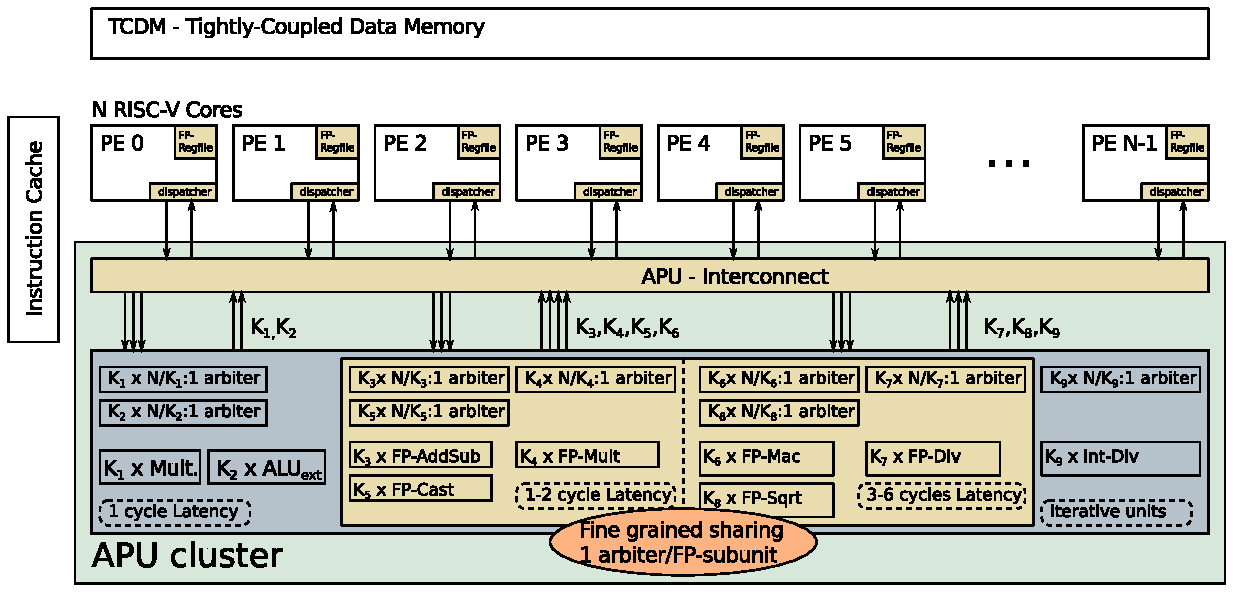
\includegraphics[height = 8cm]{figures/APU_concept.pdf}

  \vfill

  {\Large \@author}\\
  {gautschi@iis.ee.ethz.ch}
  \vfill
  \@date

 \end{center}
\end{titlepage}
\makeatother

\tableofcontents

\chapter{Overview}

The shared auxilary processing unit~(APU) is designed to work with the \rvcore core and aims on sharing expensive ISA extensions in one shared unit among all cores. \rvcore is a four-stage in-order \riscv core architecture which supports the following instructions:

\begin{itemize}
  \item Full support for RV32I Base Integer Instruction Set
  \item Full support for RV32C Standard Extension for Compressed Instructions
  \item Full support for RV32M Standard Extension for Integer Multiplication
    and Division
  \item PULP specific extensions
        \begin{itemize}
          \item Post-Incrementing load and stores
          \item Multiply-Accumulate and dot-product extensions
          \item ALU extensions
          \item Hardware Loops
        \end{itemize}
  \item Full support for RV32F Floating Point Extension through a shared or a private FPU
\end{itemize}

This document describes how the shared APU can be used, to better amortize costly instruction extensions, such as the full floating-point RV32F extension. \chref{ch:apuarchi} will detail the architecture of the shared APU including the building blocks such as arbiters, interconnects, and the shared units. \chref{ch:coreext} explains the required core extensions for interfacing the shared APU, and \chref{ch:examples} will provide information about the current functionality of the shared APU, mainly the shared dot-product instructions, and the shared FPU.

\section{Overall Sharing Concept}
The idea of sharing units is that all cores in a multi-core cluster see the shared resources as if they had private instances. Hence, to a programmer, the sharing of resources is completely transparant.
There are two distinct ideas on sharing resources as indicated in \figref{fig_apu:sharedunit}. We differentiate between a \texttt{simple sharing} and a \texttt{fine-grained sharing}. The former shares one block which itself supports different operations. This approach is typically prefered when the different subunits are not used concurrently, and they can itself share a large part of its datapath. The logarithmic number unit (LNU) \cite{Gautschi_jssc} is a good example for this sharing approach, because all operations are interpolated in a second order interpolator which is in common for all operations, but the look-up tables are different distinct.

The fine-grained sharing is more complex and does not aim to share a single unit, but directly the individual operators. This has several advantages because it allows for a fine-grained adjustment of unit instantiations (e.g. one FP-divider and 2 FP-FMA units), it allows the different types of units to have a different latency (e.g. multi-cycle FP-divisions, and two-cycle FP-additions), and it allows the cores to access the different units concurrently.
In contrast to just instantiating multiple units, this allows to better control the number of subunits, minimize the overall area consumption, and therefore use a simpler arbitration circuit (an 8:1 arbitration is faster than an 8:2 arbitration).

Supporting different latencies in the fine-grained shared unit is only possible if the interconnect can stall the different units, and cores to resolve access and write-back conflicts or if the cores know the latencies of the individual instructions and can avoid collisions before they occur. The first approach is a bit more flexible but poses additional constraints on the interconnect. This makes the interconnect more complex, but more importantly, increases the latency of the interconnect which forces to use additional pipeline registers in the units itself leading to more stalls.

For this reason, we have opted for the second option where each core is aware of the instruction latencies and only issues new instructions to the APU which have a latency which is greater or equal to the latency of the previous instruction.

In the following the fine-grained shared auxiliary processing unit~(APU), the interconnect and the core dispatcher will be explained in more detail.

\begin{figure}[t]
\centering
  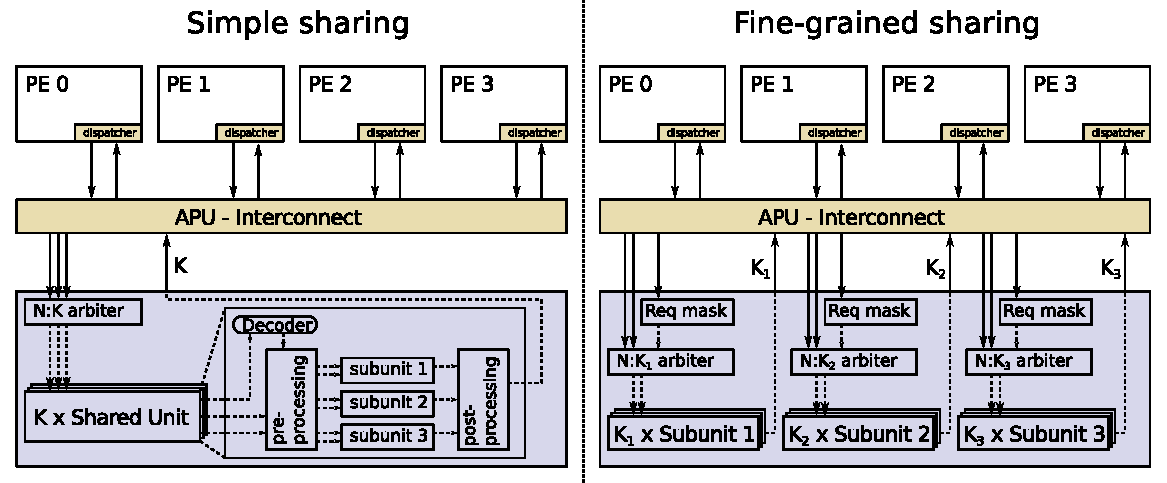
\includegraphics[width=1\linewidth]{figures/SharedUnit.pdf}
  \caption{Simple sharing: One type of unit with support of different subfunctions is shared. Fine-grained sharing: the subfunctions are shared directly.}
  \label{fig_apu:sharedunit}
\end{figure}

\chapter{The APU Architecture}\label{ch:apuarchi}

\begin{figure}[t]
\centering
  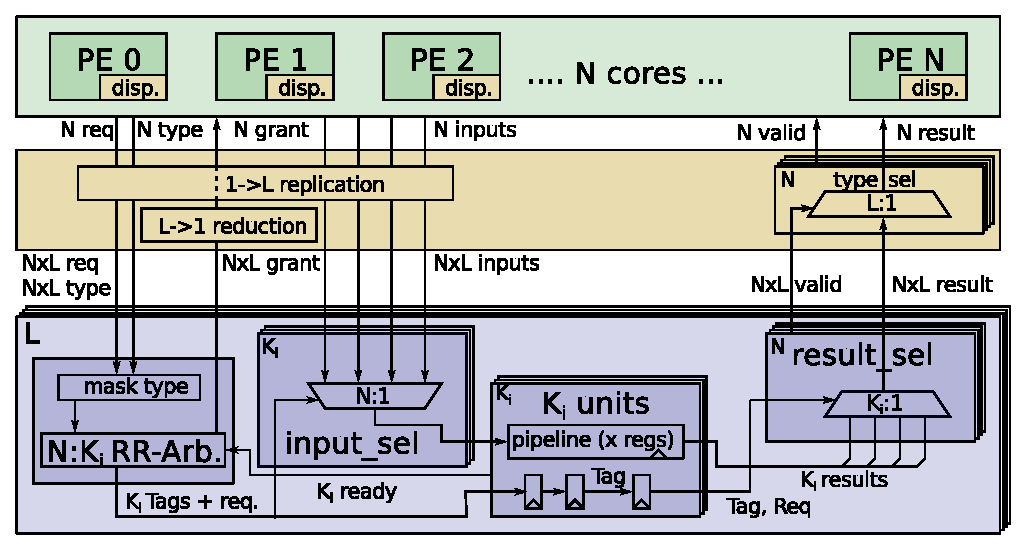
\includegraphics[width=1\linewidth]{figures/interconnect.pdf}
  \caption{Interconnect with multiple types of execution units.}
  \label{fig_apu:interconnect}
\end{figure}

This chapter deals with the interconnect in \secref{interconnect}, the shared subunits in \secref{sharedunit}, and the interface of the APU to the cores in \secref{apuinterface}.

\section{Interconnect}\label{interconnect}
As shown in \figref{fig_apu:interconnect} the task of the interconnect is to connect $N$ PEs with all $L$ types of shared execution units. Each dispatcher signals, that it wants to offload an instruction with a \texttt{request} signal. A \texttt{type} signal is used to route the instruction which consists of \texttt{operands}, \texttt{opcode}, and \texttt{flags} to the corresponding unit. For each type $L$ the \texttt{type}, \texttt{request}, \texttt{operand}, and \texttt{opcode} signals of all $N$ dispatchers have to be replicated and routed to the shared units. Each shared unit can execute one operation per PE, and hence generates $N$ \texttt{grant}, \texttt{result}, and \texttt{valid} signals which have to be routed back to the $N$ PEs. Since each PE can only issue one transaction per clock cycle, the reduction block for the \texttt{grant} is a simple logic \emph{or} of all $L$ types.
% Each results comes with a \texttt{tag} signal which identifies to which PE it has to be routed back.
If all shared units have the same latency, it is not possible that more than one result is valid at the same time. Hence, only one result needs to be selected with a $L:1$ multiplexer, and forwarded to the core.
Since it is unlikely that all shared units have the same latency, additional constraints are posed on the dispatcher to make sure that transactions of a given PE do not overtake each other or finish concurrently which would mean that multiple results would have to be routed back to the same PE in a single clock cycle. These constraints are explained in the following in more detail.

\section{Arbitration and Shared Units}\label{sharedunit}
To support a fine-grained sharing of execution units as shown in \figref{fig_apu:sharedunit}, each type requires its own arbitration unit which assigns the $K_i$ units according to the $N$ requests. Each arbiter is identified with a unique type identifier and the requests are filtered by the type before the actual arbitration is performed.
%Hence, requests are only forwarded to the arbiter if the corresponding type matches.
A simple round-robin arbiter has been used for the arbitration of $N$ cores and $K_i$ shared units.
The arbiter generates a tag that is used to identify the source. This tag is then forwarded to the \texttt{input\_sel} unit to select the right input operands, and to the actual shared unit which can be implemented as
\begin{itemize}
\item an iterative, blocking unit
\item or a pipelined unit.
\end{itemize}
\figref{fig_apu:interconnect} shows a pipelined unit with $x$ registers stages which can accept one operation per cycle, and outputs the result after $x+1$ cycles. In this case, the tag needs to propagate through a separate pipeline of the same depth. The tag can then be used in the \texttt{output\_sel} unit to select the right result and forward it to the right core. Note, because all $K_i$ units of one specific type have the same latency, and a core can only issue one operation per cycle, it is not possible that two shared units of the same type have a result for the same core. Therefore, a simple multiplexer can be used to select the output.

Iterative, blocking units are also supported, but require an additional \texttt{ready} signal to inform the arbiter whether is ready to accept a new operation or not. This \texttt{ready} signal is used by the arbiter to decline requests to this specific unit.

Cluster implementations with more than four cores likely require sharing more than one unit of each type without significantly increasing the number of access contentions. The more cores ($N$), and shared execution units ($K_i$), the more complex the arbitration, and input/output selection becomes. In fact, for such cases, a round-robin arbiter might not always be the preferred solution because its delay is too high and would lead to a frequency degradation.

The units can have different latencies and we distinguish between three groups which are:
\begin{itemize}
\item single-cycle units (combinational units) (1 cycle delay)
\item two-cycle units (2 cycles delay)
\item multi-cycle and iterative units (more than two cycles delay)
\end{itemize}
The core has to know to which group each instruction belongs in order to issue instructions correctly.

\section{APU Interface}\label{apuinterface}
The interface signals of the APU are described in \tabref{tab_apu_interface}. Each core is sending one instance of the interface type \texttt{cpu\_marx\_if()} to the APU. The handshake consists of a request, a grant, type, and valid signal. The core sends a request and holds it high as long as the shared unit answers with a grant. During this time the type signal shall not change. In the cycle in which the grant is sent to the core, the data input signals are captured and forwarded to the corresponding unit. When no contentions occur, this all happens in the same clock cycle.
Depending on the latency of the shared unit, the valid signal goes high and signals that the result and the flags are valid and can be forwarded to the core. The interconnect has no possibility to stall the write-back process because the core dispatcher is always ready to receive a result.

The widths of the type signal depends on the number of different types of shared units (NTYPE). The width of the opcode is the maximum opcode width of any shared unit. Similarly, NDSFLAGS and NUSFLAGS determine the number of up-, and down-stream flags.

\begin{table}[t]\footnotesize
\begin{threeparttable}
\renewcommand\arraystretch{0.5}
\caption{APU Interface Signals}
\centering
\label{tab_apu_interface}
\begin{tabularx}{\textwidth}{@{}l|p{1.5cm}|p{2cm}|p{7.5cm}@{}}
\toprule
\textbf{Signal Name} & \textbf{Direction} & \textbf{Width} & \textbf{Explanation}\\
\midrule
clk\_i & input &  1 & clock\\
rst\_ni & input &  1 & reset\\
\midrule
\multicolumn{4}{c}{Handshake signals (one instance per core)}\\
\midrule
cpus[i].req\_ds\_s & input & 1             & request signal of core i \\
cpus[i].type\_ds\_d & input & clog2(NTYPE) & type signal of core i to identify the type of units it wants to access\\
cpus[i].ack\_ds\_s & output & 1            & grant signal from arbiter to core i to accept a request\\
cpus[i].valid\_us\_s & output & 1          & valid signal for core i\\
\midrule
\multicolumn{4}{c}{Data signals (one instance per core)}\\
\midrule
cpus[i].operands\_ds\_d & input            & 3x32 & the three FP- or INT-operands of core i \\
cpus[i].op\_ds\_d & input & NOP            & opcode of the operation of core i\\
cpus[i].flags\_ds\_d & input & NDSFLAGS    & flags for the shared units of core i\\
cpus[i].ready\_us\_s & input & 1           & ready signal of core i (not used statically set to 1)\\
cpus[i].result\_us\_d & output & 32        & result of the shared unit for core i\\
cpus[i].flags\_us\_d & output & NUSFLAGS   & flags from the shared unit for core i\\
\bottomrule
\end{tabularx}
\end{threeparttable}
\end{table}

\chapter{Core-Extensions}\label{ch:coreext}

This chapter introduces the additional circuits in the core architecture to support shared execution units. First, the instruction decoder is explained in \secref{decoder} and \secref{dispatcher} deals with the required instruction dispatcher that guarantees in-order execution. Finally, the core interface and the available performance counters are explained in \secref{coreinterface} and \secref{coreperf}.

\section{Instruction Decoding}\label{decoder}

The decision to offload an instruction to the shared unit is generated in the instruction decoder, which is located in ID-stage. If the right signals are set, the ID-stage is then forwarding the operands, opcode, and possible flags to the APU dispatcher, rather than to the ALU, multiplier or private FPU. The decoder needs to set an enable signal to activate the dispatcher, the opcode and the type of the shared unit for this specific operation and finally the instruction latency which can either be one, two or three. Whereas one means that the shared unit is a combinational block of latency one, two means that the unit has one pipeline stage and a latency of two cycles, and three includes all other shared units with a latency greater or equal to two cycles.
Further, the assigned type signals have to match the ones of the APU. Hence, it is not enough to redefine a type signal in the instruction decoder, but it also has to be changed accordingly in the APU.

\section{APU Dispatcher}\label{dispatcher}
The APU dispatcher is a small unit located in the EX-stage that is capable of offloading operations to the shared unit, and at the same time, handling access contentions, checking for data hazards, and write-back contentions with private execution units.
To make sure that transactions in the shared units do not overtake each other, or finish at the same time causing a write-back contention, each instruction has been annotate with a latency of one, two, or many cycles. This allows the dispatcher to know instead of speculate whether it can issue more instructions in the next cycle or needs to stall to avoid contentions. If the dispatcher issued a one or two-cycle operation, it can issue more instructions because the pipeline can hide latencies up to two cycles by using the two WB ports. Single-cycle operations can be treated as ALU operations and can write-back on the first WB port which is already used by the ALU. Two-cycle operations on the other hand are writing back on the second WB port which is also used by the LSU when loading bytes from memory. Finally, three and more cycle instructions will stall the pipeline to avoid having too many outstanding transactions.

\figref{fig_apu:insn_stream} shows six different scenarios that show what instruction sequences will force the dispatcher to stall the pipeline. The notation \texttt{APU 2} means that the instruction will be executed on the APU and will take two cycles and \texttt{wb 2} means that this instruction is written back on the second WB port.
\figref{fig_apu:insn_stream}\,a) shows how four two-cycle instructions are processed without stalls. Even when interleaved with a load operation, which takes two cycles as well, no stalls occur. \figref{fig_apu:insn_stream}\,b) then shows how a three-cycle APU instruction results in one stall cycle because the subsequent two-cycle instruction would finish at the same time, which cannot be handled by the interconnect. This collision is prevented by stalling the pipeline for one cycle.
\figref{fig_apu:insn_stream}\,c) shows how an APU access-contention results in a stall. The IF-, ID-, and EX-stage will be stalled and the APU-request will be sent until it is granted. Once granted, the next instruction can enter the EX-stage. \figref{fig_apu:insn_stream}\,d) shows that the pipeline needs to be stalled for two cycles in case a three-cycle APU instruction is followed by a single-cycle APU instruction. Without stalling in such situations, the instructions would be written back OOO, which would complicate exception handling, debugging, and hazard detection.

\begin{figure}[t]
\centering
  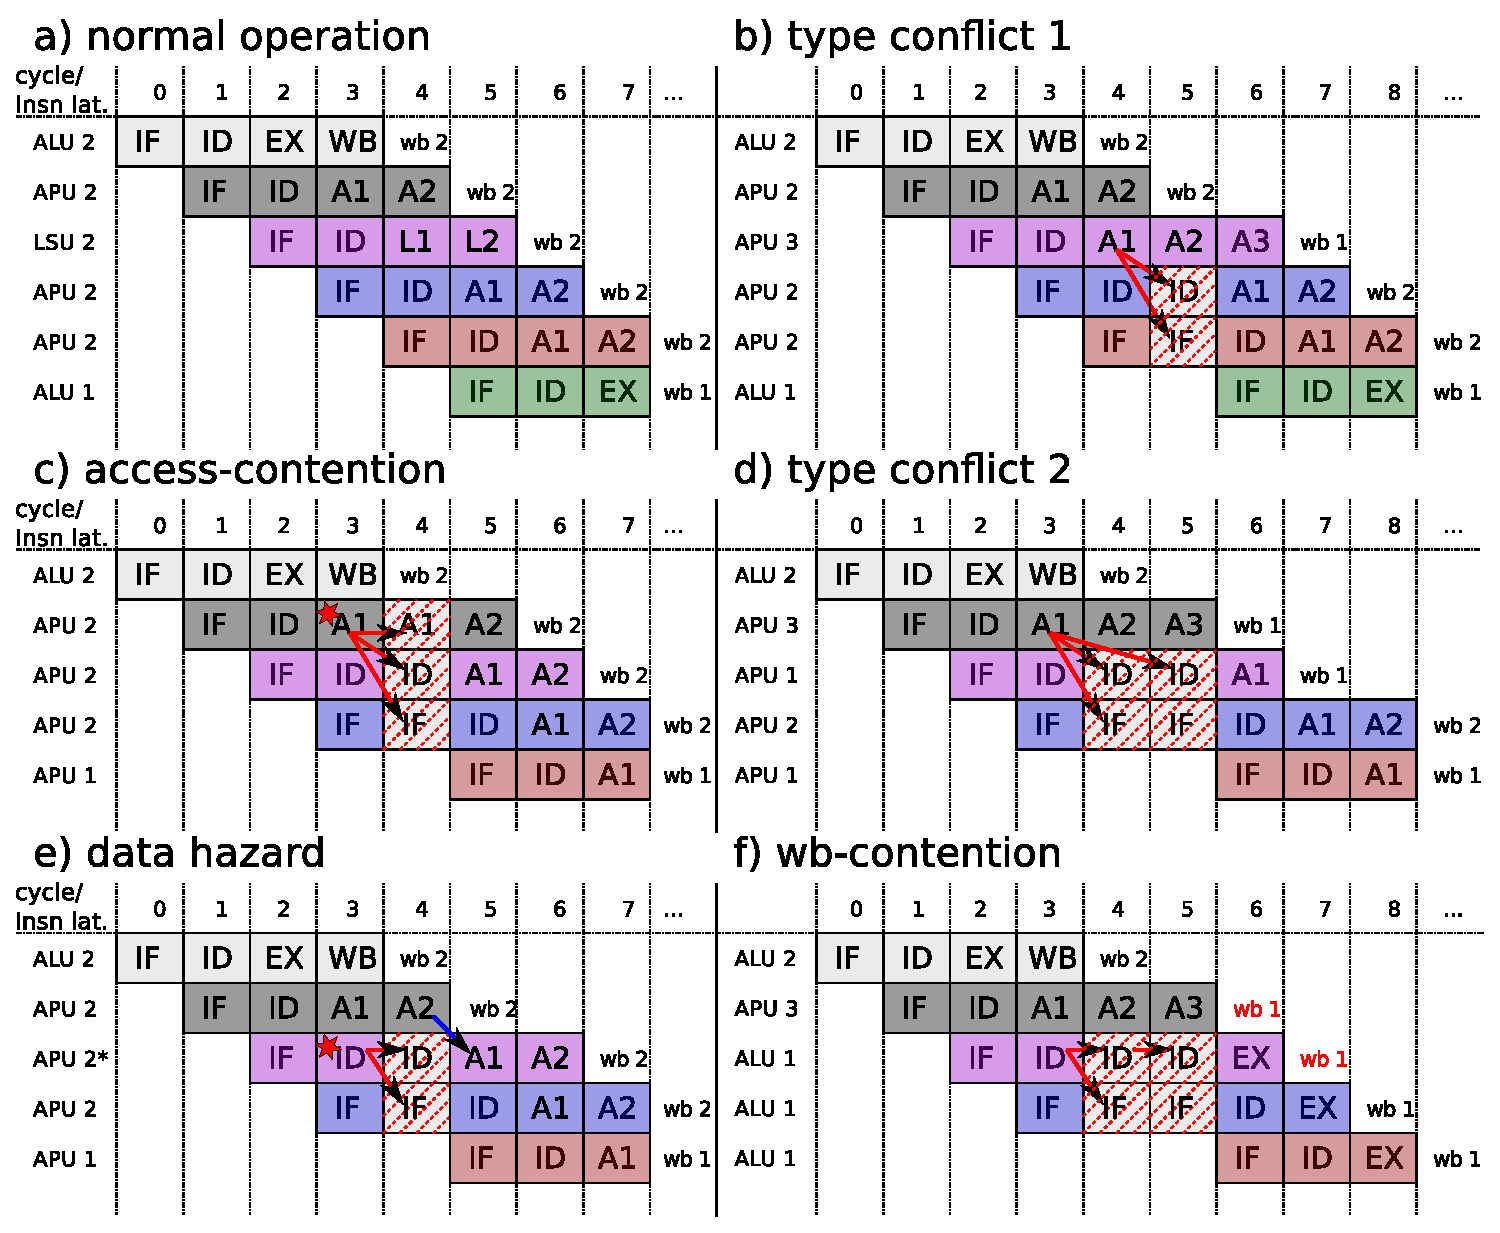
\includegraphics[width=0.99\linewidth]{figures/insn_stream.pdf}
  \caption{Example of six different scenarios when dealing with variable latency APU instructions. a) shows a series of contention free two-cycle APU instructions which execute without stalls whereas the other scenarios lead to stalls due to variable latency, data hazards, access contentions and WB contentions.}
  \label{fig_apu:insn_stream}
\end{figure}

Even if the three-cycle APU instruction was followed by another APU instruction which takes three cycles (or even more), the dispatcher stalls the pipeline, because otherwise the dispatcher needs to check for dependencies versus yet another instruction. This would require additional comparators and make the control logic much more complex.
Note, as multi-cycle instructions are typically less frequent, it is highly unlikely that two such instructions are executed in a row. Moreover, it is unlikely that the two instructions do not depend on each other. Hence, this limitation does not result in a significant performance degradation. Due to the increased complexity, and the very rare use-case, the dispatcher does not support OOO APU instructions.
\figref{fig_apu:insn_stream}\,e) shows how a data hazard is detected when decoding the instruction \texttt{APU 2*} which depends on the previous instruction. This is handled the same way as for any other instruction and will stall the pipeline to resolve the hazard. This hazard detection will not only stall the pipeline but also forward the result of the previous instruction to the current one as indicated by the blue arrow. Finally, \figref{fig_apu:insn_stream}\,f) shows that if an ALU instruction follows a multi-cycle APU instruction both want to write back the result on the first WB port which will lead to stalls first to prevent OOO WB and second to resolve the WB contention.

\section{Core Interface}\label{coreinterface}

\tabref{tab_core_interface} describes the core interface signals which are used to interface the shared APU. The meaning of the signals is identical to the one described in \secref{apuinterface}. Note that the parameters NTYPE, NDSFLAGS, NUSFLAGS, NOP have to match the one of the APU.


\begin{table}[t]\footnotesize
\begin{threeparttable}
\renewcommand\arraystretch{0.5}
\caption{Core Interface Signals to interface the APU}
\centering
\label{tab_core_interface}
\begin{tabularx}{\textwidth}{@{}l|p{2cm}|p{2.3cm}|p{6cm}@{}}
\toprule
\textbf{Signal Name} & \textbf{Direction} & \textbf{Width} & \textbf{Explanation}\\
\midrule
\multicolumn{4}{c}{Handshake signals}\\
\midrule
apu\_master\_req\_o & output & 1             & request signal \\
apu\_master\_type\_o & input & clog2(NTYPE)  & type signal to identify shared unit\\
apu\_master\_gnt\_i & output & 1             & grant signal from arbiter\\
\midrule
\multicolumn{4}{c}{Request channel}\\
\midrule
apu\_master\_operands\_o & output            & 3x32 & the three FP- or INT-operands\\
apu\_master\_op\_o & output & NOP            & opcode of the operation\\
apu\_master\_flags\_o & output & NDSFLAGS    & flags for the shared units\\
\midrule
\multicolumn{4}{c}{Response channel}\\
\midrule
apu\_master\_valid\_o & output & 1           & valid signal\\
apu\_master\_result\_i & input & 32          & result of the shared unit\\
apu\_master\_flags\_i & input & NUSFLAGS     & flags from the shared unit\\
\bottomrule
\end{tabularx}
\end{threeparttable}
\end{table}


\section{APU Performance Counters}\label{coreperf}

\tabref{tab_perf_counters} summarizes the available performance counters which can be used to profile applications which use the shared APU. The four different counters correspond to the events described in \figref{fig_apu:insn_stream} of \secref{dispatcher}. \figref{fig_apu:insn_stream}\,b), and d) will trigger an APU\_TYPE conflict and \figref{fig_apu:insn_stream}\,c) triggers the APU\_CONT counter. \figref{fig_apu:insn_stream}\,e) increases the APU\_DEP counter, and \figref{fig_apu:insn_stream}\,f) the APU\_WB counter.

As for all other performance counters, on a ASIC target only one counter exists but can be configured to count any event.

\begin{table}[t]\footnotesize
\begin{threeparttable}
\renewcommand\arraystretch{0.5}
\caption{Available Performance Counters to Profile the Shared APU}
\centering
\label{tab_perf_counters}
\begin{tabularx}{\textwidth}{@{}l|p{10cm}@{}}
\toprule
\textbf{Performance Counter Name} & \textbf{Explanation}\\
\midrule
APU\_CONT   & APU access contention: This counter is triggered when more than one core is trying to access the same shared subunit and is not getting the resource. It is a very similar type of contention to TCDM contentions.\\
\midrule
APU\_TYPE   & This counter is triggered when the latency of the current instruction is smaller than the one of a pending APU instruction. The dispatcher stalls in these cases and prevents write back collisions in the interconnect.\\
\midrule
APU\_DEP    & APU inter-instruction dependencies: These stalls occur when the result of an APU instruction is not yet ready but required by the current instruction.\\
\midrule
APU\_WB     & APU write-back contentions. Although, write-back contentions are avoided in the dispatcher, they can still occur with private ALU operations and multiplications which are single-cycle operations. If a multi-cylce APU operation wants to write back its result and a ALU operation entered the pipeline, it might be that they both want to commit at the same time which will stall the ALU operation for one cycle.\\
\bottomrule
\end{tabularx}
\end{threeparttable}
\end{table}

\chapter{Available Functionality}\label{ch:examples}

Different shared units have been tested and the most promising candidates are available in the PULP cluster. The shared APU can be configured with a set of parameters which are defined in a single package (\texttt{apu\_package.sv} located in rtl/ulpcluster).

\begin{itemize}
\item \textbf{FPU:}\\ when set to one, the core is extended with floating-point capabilities.
\item \textbf{SHARED\_FP:}\\ when set to one, the FP-signals are connected to the APU rather than to a private FPU. The shared FP-operators are instantiated in the APU.
\item \textbf{SHARED\_DSP\_MULT:}\\ when set to one, the dot-product extensions are moved to the APU.
\item \textbf{SHARED\_INT\_DIV:}\\ when set to one, the integer divider is moved to the shared APU.
\item \textbf{SHARED\_INT\_MULT:}\\ when set to one, the integer multiplier is moved to the shared APU.
\item \textbf{SHARED\_FP\_DIVSQRT:}\\ defines what kind of FP-DIV/SQRT unit is instantiated.
\end{itemize}

The SHARED\_INT\_DIV, and SHARED\_INT\_MULT parameters are set to zero by default because the amount of saved area due to sharing is small compared to the others. More detailed configuration results are provided for the shared dot-product unit in \secref{apu_dsp} and the shared FPU in \secref{apu_fpu}.

\section{Shared DSP Units}\label{apu_dsp}

The first sharing candidates are the dot-product extensions as one of these units alone consumes 6.5\kGE and increases the core area significantly. Dot-product units allow the core to compute up to four multiplications and four accumulations in one cycle which can significantly speed up compute-intensive kernels and at the same time reduce load/store bandwidth. In the most dot-product intense benchmarks (convolutions, matrix multiplications) the utilization of the dot-product unit is between 10\% and 30\%, making them perfect candidates to be shared in the APU with either one single or two subunits.

\begin{figure}[t]
\centering
  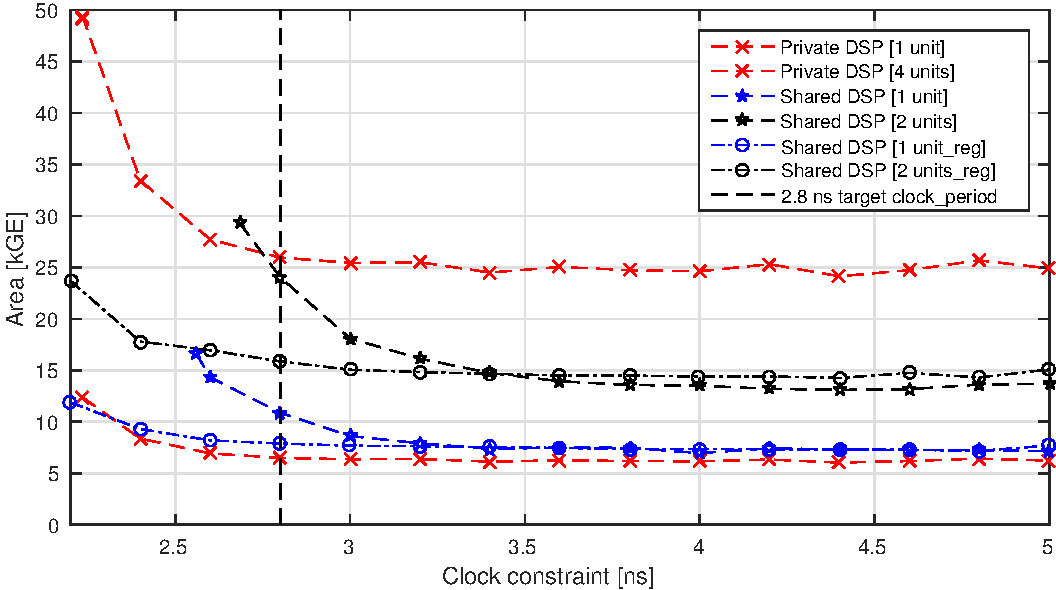
\includegraphics[width=0.95\linewidth]{figures/AT_dsp_units.pdf}
  \caption{Private versus shared dot-product units for a four-core cluster. Shared configurations with one, and two subunits are shown with and without a pipeline stage.}
  \label{fig_apu:dsp_at}
\end{figure}

Since dot-product instructions are often used in back-to-back fashion, these units have been designed to complete in one cycle. In a shared context, these units will require some extra timing margin for the arbitration between all cores. Since these units were already close to be timing critical, the area-delay behavior of four shared DSP configurations has been evaluated in \figref{fig_apu:dsp_at} to determine if an additional pipeline stage is necessary using a 65nm UMC technology node.
The plot shows the area of one and four dot-product units for the private case and one or two dot-product units with one or none pipeline stage for the shared configuration. At a target clock period of 2.8\ns for this technology node, the private dot-product units consume 26\kGE, four times more than a single instance. Sharing only one dot-product unit is the cheapest option, but might lead to many access contentions. Due to the additional area requirement of the $4:1$ arbiter, one shared dot-product unit is always larger than a private dot-product unit, but only 1\kGE. However, sharing a dot-product unit not only increases the dot-product unit by 1\kGE but requires 11\kGE due to the additional timing pressure. Adding a pipeline register to the dot-product unit results in a smaller area but also decreases performance due to the increased latency. Hence, for a single unit, an additional pipeline register can be beneficial but is not yet necessary.

The conclusion changes when more than just one shared unit is required. In this case, the pipelined version is 8\kGE smaller than a single cycle unit because it is much less timing critical. Hence, when sharing more than one unit, it is more area efficient to use a pipelined dot-product unit. Such a pipelined unit increases the delay of each dot-product instruction, which can be hidden in most applications by simply using two independent accumulation registers and interleaving the dot-product instructions. \tabref{tab_apu:conv_opt} shows the generated assembly of the inner loop of a 5x5 convolution kernel on byte elements. Five dot-product and sum-of-dot-product instructions are required to perform the 25 multiplications per pixel. In this example, registers \texttt{r3\,-\,r9} are used to store the weights, and registers \texttt{r12\,-\,r18} contain the current values of the image patch. The assembly instructions on the left hand side were generated by a convolution with only one accumulation register (\texttt{r19}). Five of the seven sum-of-dot-product instructions have dependencies amongst themselves and will stall the core whereas the assembly on the right hand side of \tabref{tab_apu:conv_opt} was generated with two distinct and interleaved accumulation registers (\texttt{r19,r20}). This interleaved access allows to resolve any kind of inter-instruction dependencies. In the end, the two accumulation registers have to be summed up which can even be merged with a round and normalize instruction allowing to perform a convolution without additional stalls and without increasing the number of instructions. The only source for stalls when sharing dot-product units are access contentions at the shared unit.
%
With respect to a private implementation, the shared architecture allows to save 10\,-\,18\kGE depending on the number of required units.


\subsection{Options}
The pipeline depth and the number of dot-products units can be adjusted in the APU. In order to do so, the parameters in the APU cluster package (\texttt{apu\_cluster\_package.sv} located in apu\_cluster/sourcecode) can be modified. The parameter \texttt{C\_DSP\_PIPE\_REGS} sets the amount of pipeline registers. By default, one pipeline register is inserted which means that dot-product instructions take two cycles in total. If no pipeline stage is desired, this parameter can be set to 0 which will make dot-product instruction single-cycle. By doing this, the latency parameter in the core has to be adjusted accoringly.

The number of units can be controlled with the parameter \texttt{NAPUS\_DSP\_MULT} which is set in the top level file of the APU (\texttt{apu\_cluster\_no\_bid\_if.sv}). For DSP intensive programs a value of N/2 has found to be optimal, where N is the number of cores. If the unit is not intended to be used very often, it can be set to one.

\subsection{Instruction Latencies and Usage in C}

The sharing is completely transparent which means that no special care is required when programming. The additional latency of the dot-product unit can however lead to more depenency stalls which can be prevented in most kernels by hiding the latency of these operations. The following example in \tabref{tab_apu:conv_opt} provides an example of utilizing two independent accumulation registers which allow to process dot-product instructions without any stalls.

\begin{table}[t]\footnotesize
\begin{threeparttable}
\renewcommand\arraystretch{0.5}
\caption{5x5 convolution with and w/o interleaved accumulations.}
\centering
\label{tab_apu:conv_opt}
\begin{tabular*}{\columnwidth}{l@{\extracolsep{\fill}}*{2}{l}}
\toprule
Convolution with one accumulator & Convolution with two accumulators \\
\midrule
  \texttt{...}                                   & \texttt{...}                                          \\
  \texttt{start of inner iteration  }            & \texttt{start of inner iteration  }                   \\
  \texttt{...}                                   & \texttt{...}                                          \\
  \texttt{pv.dotp.b~~~\green{r19},~r12,~r3~~}    & \texttt{pv.dotp.b~~~\green{r19},~r12,~r3~~}           \\
  \texttt{pv.sdotp.b~~\red{r19},~r13,~r4~~}      & \texttt{\blue{pv.dotp.b}~~~\blue{r20},~r13,~r4~~}     \\
  \texttt{pv.sdotp.b~~\red{r19},~r14,~r5~~}      & \texttt{pv.sdotp.b~~\green{r19},~r14,~r5~~}           \\
  \texttt{pv.sdotp.b~~\red{r19},~r15,~r6~~}      & \texttt{pv.sdotp.b~~\blue{r20},~r15,~r6~~}            \\
  \texttt{pv.sdotp.b~~\red{r19},~r16,~r7~~}      & \texttt{pv.sdotp.b~~\green{r19},~r16,~r7~~}           \\
  \texttt{pv.sdotp.b~~\red{r19},~r17,~r8~~}      & \texttt{pv.sdotp.b~~\blue{r20},~r17,~r8~~}            \\
  \texttt{lw~~~~~~~~~~r17,~-4(r23)~}             & \texttt{lw~~~~~~~~~~r17,~-4(r23)~}                    \\  
  \texttt{pv.sdotp.b~~\green{r19},~r18,~r9~~}    & \texttt{pv.sdotp.b~~\green{r19},~r18,~r9~~}           \\
  \texttt{p.lb~~~~~~~~r18,~r24(r23!)~}           & \texttt{p.lb~~~~~~~~r18,~r24(r23!)~}                  \\  
  \texttt{p.addrn~~~~~r19,~\green{r19},~zero,~6} & \texttt{p.addrn~~~~~r19,~\green{r19},~\blue{r20},~6}  \\
  \texttt{p.clipu~~~~~r21,~r19,~7~~~~~~}         & \texttt{p.clipu~~~~~r21,~r19,~7~~~~~~}                \\
  \texttt{...}                                   & \texttt{...}                                          \\
  \texttt{move and shuffle elements}             & \texttt{move and shuffle elements}                    \\
  \texttt{...}                                   & \texttt{...}                                          \\
\bottomrule
\end{tabular*}
\end{threeparttable}
\end{table}


\section{Shared FPU}\label{apu_fpu}

Since floating point extensions come at a non-negligible cost, and due to the reason that FPUs are never fully utilized, it makes sense to share the FP-operators in the APU. The fine-grained sharing concept of the APU is perfectly suited to build a scalable FPU for multi-core clusters like PULP. Since the latency of the individual instructions are different, the operations can be grouped in different types which can be accessed concurrently. Further, by sharing the operators, rather than a full FPU allows to better balance the number of units. Finally, by sharing the operators itself, the total number of units can be minimized (usually to one) because the cores can access the different types concurrently.


\begin{table}[t]\footnotesize
\begin{threeparttable}
\renewcommand\arraystretch{0.5}
\caption{Available FPU configuration options.}
\centering
\label{tab_apu:fpuoptions}
\begin{tabularx}{\textwidth}{@{}l|x{2cm}x{2cm}x{3cm}|x{1.5cm}x{1.5cm}@{}}
\toprule
\textbf{Configurations} & \multicolumn{3}{c|}{\textbf{Parameter names}} & \multicolumn{2}{c}{\textbf{Est. Area [kGE]}}\\
&\textbf{\texttt{FPU}} & \textbf{\texttt{SHARED\_FP}} & \textbf{\texttt{SHARED\_FP\_DIVSQRT}} & per core & per cluster\\
\midrule
\multicolumn{6}{c}{\textbf{Private Configurations}} \\
\midrule
\midrule
\textbf{No FP Support} & 0 & 0 & 0 && \\
\midrule
Units/area per core & \multicolumn{3}{c|}{none} & 0 & 0 \\
\midrule
\midrule
\textbf{Private FPU 1}& 1 & 0 & 0 && \\
\midrule
Units/area per core & \multicolumn{3}{c|}{1 FPU (ADD, MUL, CAST), 1 FMA} & 23 & N$\times$23\\
\midrule
\midrule
\textbf{Private FPU 2}& 1 & 0 & 2 && \\
\midrule
Units/area per core & \multicolumn{3}{c|}{1 FPU (ADD, MUL, CAST), 1 FMA, 1 iter. DIV/SQRT} & 30 &N$\times$30\\
\midrule
\multicolumn{6}{c}{\textbf{Shared Configurations}} \\
\midrule
\midrule
\textbf{Shared FPU 1}& 1 & 1 & 0 && \\
\midrule
Units/area per cluster & \multicolumn{3}{c|}{1 ADD, 1 MUL, 1 CAST, 1 FMA} & - & 27 \\
\midrule
\midrule
\textbf{Shared FPU 2}& 1 & 1 & 1 && \\
\midrule
Units/area per cluster & \multicolumn{3}{c|}{1 ADD, 1 MUL, 1 CAST, 1 FMA, 1 DIV, 1 SQRT } & - & 56\\
\midrule
\midrule
\textbf{Shared FPU 3}& 1 & 1 & 2 && \\
\midrule
Units/area per cluster & \multicolumn{3}{c|}{1 ADD, 1 MUL, 1 CAST, 1 FMA, 1 iter. DIV/SQRT } & - & 34\\
\midrule
\midrule
\textbf{Not supported} & \multicolumn{3}{c|}{all other combinations} & \\
\bottomrule
\end{tabularx}
\end{threeparttable}
\end{table}


\subsection{Options}
The current cluster supports six different floating point options which are summarized in \tabref{tab_apu:fpuoptions}. The first option does not support FP operations, and the other five support single-precision FP operations with different number and type of hardware units. The private options come with support for ADD, MUL, CAST through one single unit with an optional support for iterative DIV/SQRT operations. The shared options come with an additional FMA unit, and with different flavours of DIV, SQRT support. Shared FPU 1 does not support DIV/SQRT, Shared FPU 2 supports these operations through a pipelined unit, and Shared FPU 3 with the iterative DIV/SQRT unit.

The number of pipeline registers of the different FP-operators can be controlled with the parameters \texttt{C\_*\_PIPE\_REGS} in the package (\texttt{apu\_cluster\_package.sv} located in apu\_cluster/sourcecode/).

The number of instantiated FP-operator units can be set in the toplevel file of the APU with the parameters \texttt{NAPUS\_*}.



\subsection{FP Register File}

By default FP operands are located in an own register file which is implemented on top of the integer register file as illustrated in \figref{fig_apu:regfile}. A merge of the two register files is possible with the restriction that FP register r0 is always 0.0F. The compiler needs to be aware of this merge.

\begin{figure}[tb]
\centering
  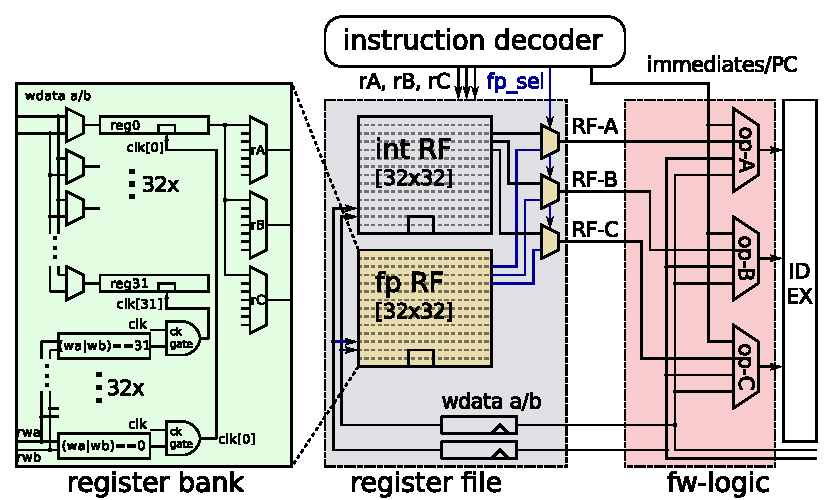
\includegraphics[width=0.95\linewidth]{figures/rf_fpu.pdf}
  \caption{Fused integer and floating point register file.}
  \label{fig_apu:regfile}
\end{figure}


\subsection{DW Components}

For the fine-grained shared FPU, individual operators are prefered over shared units. Since the DW library of Synopsys (or other vendors) offer high quality FP operators, such units are ideally suited to build a shared FPU. On the other hand, single core configurations, where only one operation can be carried out concurrently, prefer a fused data path.
DW components come as combinational blocks and are instantiated with a configurable number of pipeline registers either at the input or output of the unit. To achieve an optimal frequency, these registers have to be retimed. Utilizing Synopsys Design Compiler, the following command can be used to retime all FP wrappers:

\begin{itemize}
\item [DC>] set\_optimize\_registers -designs [get\_designs cluster\_fp\_wrap*]
\end{itemize}

By sourcing this command before the actual compilation, \texttt{compile\_ultra} will retime the specified designs in the mapping stage.

\subsubsection{Reference Area and Delay Results}
\figref{fig_apu:at_fp_units} shows an AT curve of different parametrized DW components when retimed in a 65nm technology and \tabref{tab_apu:fp_units} summarizes the different area consumption and instruction latencies of all FP components at a frequency matching the \rvcore core. The latencies of the individual instructions can be changed by adding/removing pipeline stages to the units as explained earlier.

\begin{figure}[t]
\centering
  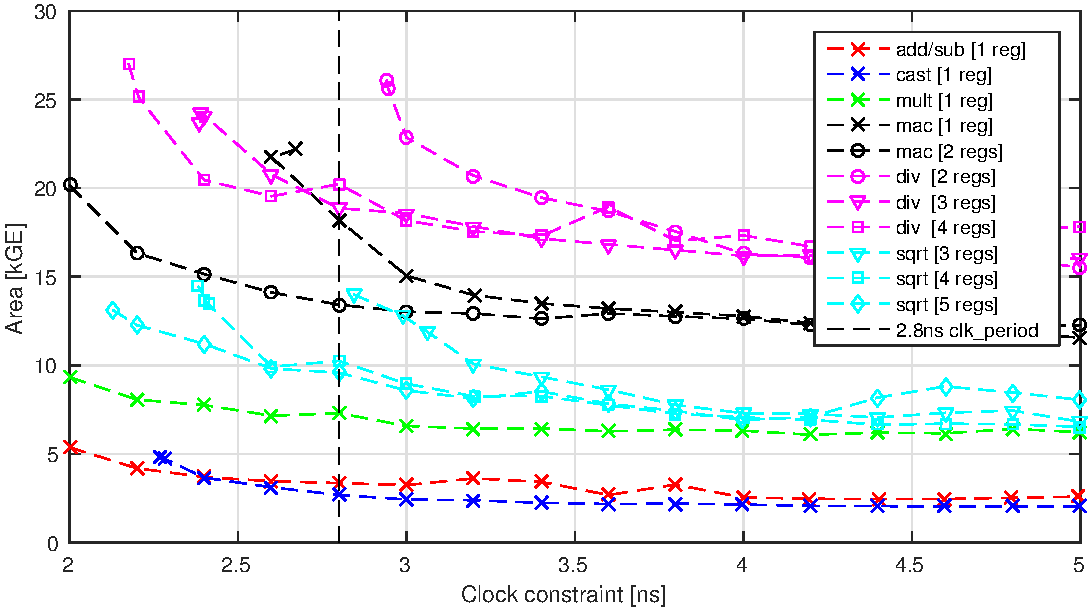
\includegraphics[width=0.95\linewidth]{figures/AT_FP_units.pdf}
  \caption{Area-delay trade-off of different \riscv FP components.}
  \label{fig_apu:at_fp_units}
\end{figure}

\begin{table}[t]\footnotesize
\begin{threeparttable}
% increase table row spacing, adjust to taste
\caption{Area-delay trade-off of different Synopsys DW FP-operators with a 2.8ns clock period and 0.5ns input/output delay. (UMC 65nm, 1.08V, worst-case conditions)}
\label{tab_apu:fp_units}
\centering
\begin{tabularx}{\textwidth}{@{}lp{0.5cm}|x{1.4cm}x{1.3cm}x{0.7cm}x{1.3cm}@{}}
\toprule
\multicolumn{2}{@{}l|}{\multirow{2}*{FP-Operator}}               & \textbf{Pipeline}           & \textbf{Latency}          & \multicolumn{2}{c}{\textbf{Area [kGE]$^a$}} \\
                                           &                     & \textbf{registers}          & \textbf{[Cycles]}         & DW   & FPU\\  
\midrule
ADD/SUB                                    & hw                  & 1                           & 2                         & 3.4  & \multirow{3}*{9.6} \\
MULT                                       & hw                  & 1                           & 2                         & 7.3  &                    \\
I2F, F2I                                   & hw                  & 1                           & 2                         & 2.7  &                    \\
\midrule
\multirow{2}*{FMA}                         & \multirow{2}*{hw}   & 1                           & 2                         & 18.2 & \multirow{2}*{-}   \\
                                           &                     & 2                           & 3                         & 13.4 &                    \\
\midrule
\multirow{4}*{DIV}                         & \multirow{2}*{hw}   & 3                           & 4                         & 18.9 & \multirow{2}*{-}   \\
                                           &                     & 4                           & 5                         & 19.5 &                    \\
                                           & hw               & -                           & 8$^b$                         & -    &  7.0$^c$          \\
                                           & sw                  & -                           & ~65                       & -    & -                  \\
\midrule
\multirow{5}*{SQRT}                        & \multirow{3}*{hw}   & 3                           & 4                         & 14.0 & \multirow{3}*{-}   \\
                                           &                     & 4                           & 5                         & 10.2 &                    \\
                                           &                     & 5                           & 6                         & 9.6  &                    \\
                                           & hw               & -                           & 8$^b$                         & -    &  7.0$^c$           \\
                                           & sw                  & -                           & 50                        & -    & -                  \\
%
\bottomrule
\end{tabularx}
\begin{tablenotes}\scriptsize
\item[$^a$] 1 GE = 1.44\,\textmu m$^2$, $^b$ iterative, blocking unit, $^c$ Uses the same hardware for DIV and SQRT
\end{tablenotes}
\end{threeparttable}
\end{table}



\chapter{Future Extensions}\label{ch:future}

Finally, the APU is not limited to the presented extensions, but can be extended with more shared operators. If the following constraints are fullfilled, the ISA extension can be mapped to the APU:
\begin{itemize}
\item Not more than three 32b inputs are required.
\item The operation does generate an output of maximum 32b.
\item The operation only depends on the inputs provided by the cores, and does not rely on other inputs.
\end{itemize}

\section{How to move new instructions to the APU}

To extend the APU with a new operation, the following steps have to be carried out on cluster level (Global), APU level (APU), and in the core (Core):

\begin{enumerate}
\item [Global:]
\item Define a new instruction format in the ISA and modify the compiler accordingly.
\item Increase the parameter C\_APUTYPES by the number of additional types (see \texttt{apu\_package.sv}:  \texttt{C\_APUTYPES} has to be equal to the total number of active types)
\item [APU:]
\item Assign new and unique type identifiers for the new instructions in the APU top level file (see \texttt{apu\_cluster\_no\_bid\_if.sv}).
\item Add the desired unit to the APU, add an arbiter, and an interface to connect the arbiter with the shared unit (copy paste from any other shared module).
\item Overwrite the default parameter (\texttt{APUTYPE}) of the arbiter (marx) with the previously defined type identifier.
\item [Core:]
\item Decode the instruction in the instruction decoder. Assign the signals \texttt{apu\_en, apu\_type\_o, apu\_op\_o, apu\_lat\_o, apu\_flags\_o}. Make sure that the type matches the one in the \texttt{apu\_cluster\_no\_bid\_if.sv} (best practice is to pass it as a parameter).
\item Depending on the latency of the instruction set the \texttt{apu\_lat\_o} signal to \texttt{1} (combinational unit), \texttt{2} (one pipeline register), \texttt{3} (multi-cycle instruction).
\end{enumerate}

\begin{thebibliography}{100}

\bibitem{Gautschi_jssc}
M.~Gautschi \emph{et~al.}, ``{An Extended Shared Logarithmic Unit for Nonlinear
  Function Kernel Acceleration in a 65-nm CMOS Multicore Cluster},'' \emph{IEEE
  J. Solid-State Circuits}, vol.~52, no.~1, pp. 98--112, 2017.


\end{thebibliography}

\end{document}
